%!TEX root = ../report.tex

\begin{document}
    \chapter{Methodology}
	\label{chap:methodology}
	
	Methodology section contains the details about the dataset used for performing the experiments, preprocessing of the dataset, and experimental design.

    \section{Dataset}
    
    To conduct the experiments Scannet and Virtual KITTI 2 are used. Scannet is a indoor scenes. These dataset contains the continuous video sequence data and explained in details in the below section. 
    
    \subsection{ScanNet \ref{90_dai2017scannet}}
    
    ScanNet is a video sequence dataset with 1513 scanes captured in 707 distinct spaces. The dataset contains totally 2.5M RGB-D images. The dataset originally designed for the task of indoor scenes 3D reconstruction including 3D objec classification, semantic voxel labeling and CAD model retrieval \ref{90_dai2017scannet}, \ref{91_ScanNet}. The dataset contains the details of the 3D camera poses, surface reconstruction, and instance-level semantic segmentation. One sample of the data is shown in the figure     

	\begin{figure}[h]
		\centering
		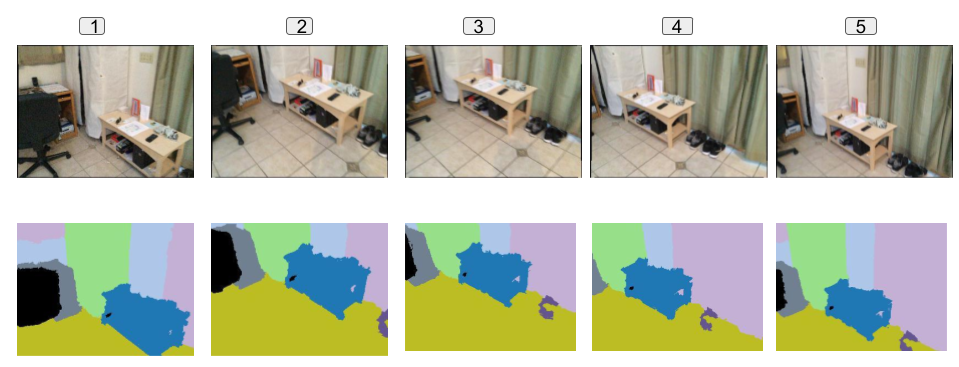
\includegraphics[width=17cm]{images/images_segm_scannet.png}
		\caption{Sample of Scannet dataset rgb and semantic label}
		\label{fig:sample_rgb_seg_scannet}
	\end{figure}
	
	\begin{figure}[h]
		\centering
		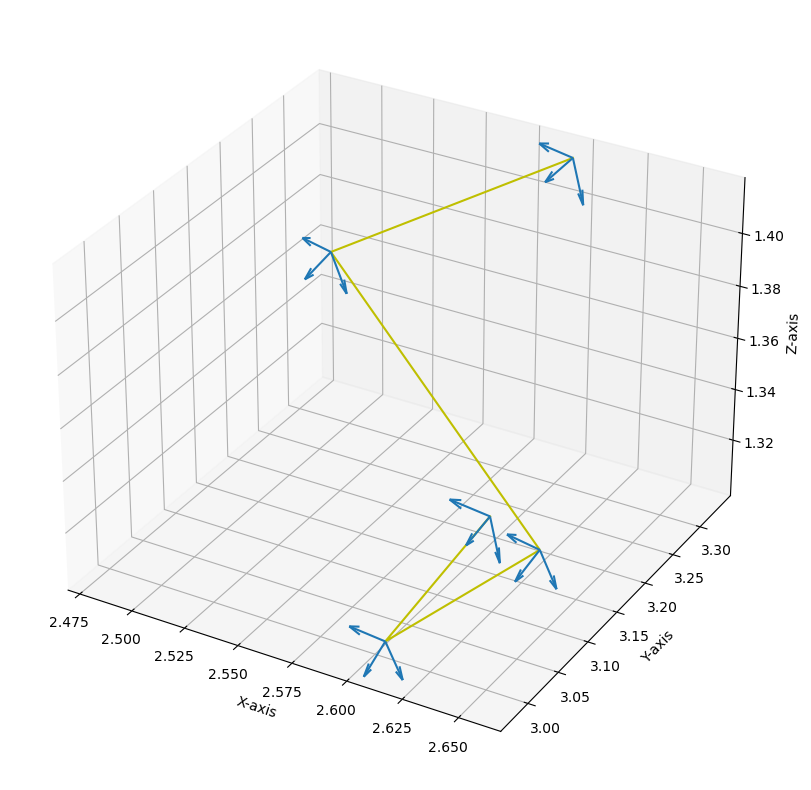
\includegraphics[width=11cm]{images/pose_viz_scannet.png}
		\caption{Sample of Scannet dataset pose}
		\label{fig:sample_pose_scannet}
	\end{figure}
	
	The 3D representation of the sample data is presented in the figure\ref{fig:sample_pose_scannet}. There are totally 40 classes in the dataset with different varieties under each categories. The complete list of the classes is presented in the Table \ref{table:Classes in scannet_1}, \ref{table:Classes in scannet_2}, and \ref{table:Classes in scannet_3}. Dataset is collected by 20 users at different countries locations. Since the dataset is huge, a subset of the dataset is taken for performing the experiments. Totally 186 video sequence data is taken for conducting the experiments. These video sequence data are further split into 149 sequence for training the model and 36 sequences for testing. The distribution of the scannet dataset labels is shown in the figure \ref{fig:scannet_class_distribution}. There is high number of pixels in the dataset belonging to the Wall, Other, Floor and Chair categories. The dataset represent the indoor scenes with different varieties. Hence experiments are conducted by combining the low pixel distribution class into a single categories to balance the pixel distribution. 
	
	\begin{figure}
		\centering
		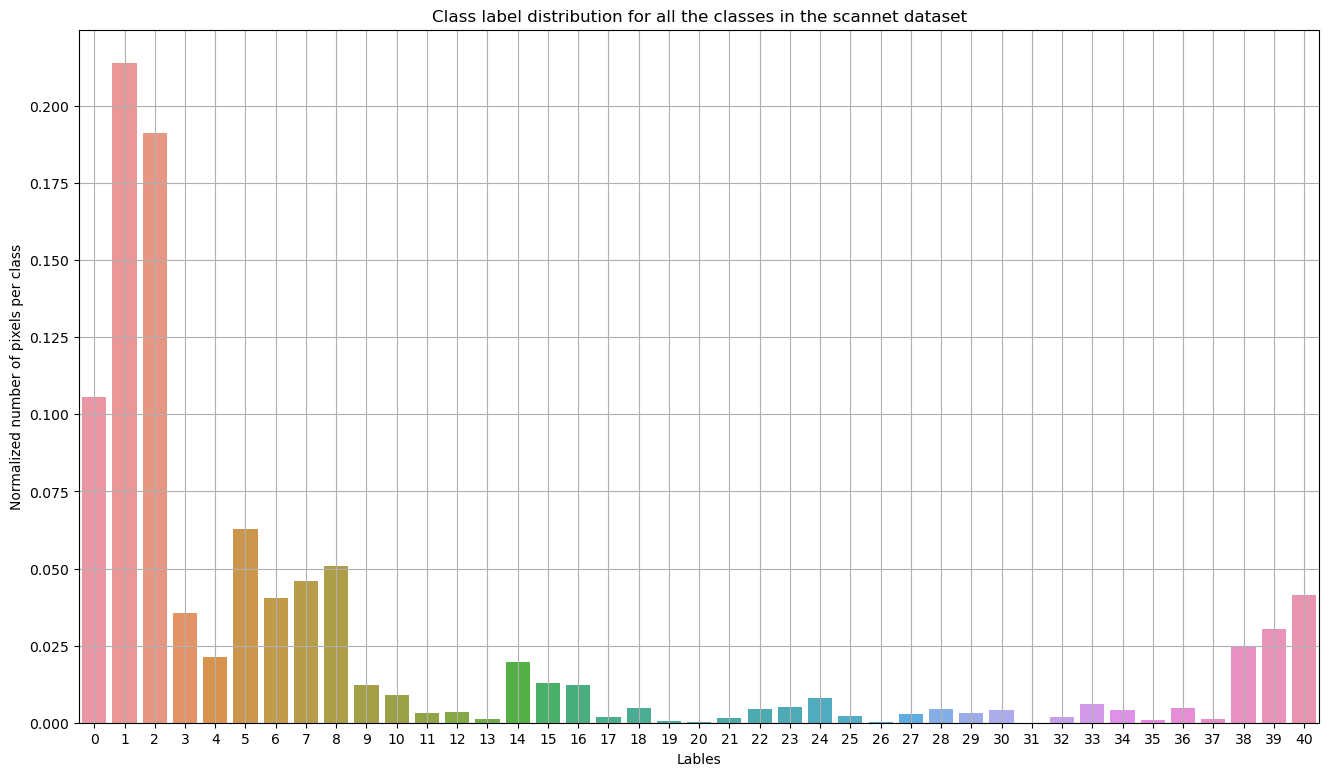
\includegraphics[width=11cm]{images/scannet_data_class_distribution.png}
		\caption{Scannet dataset class distribution}
		\label{fig:scannet_class_distribution}
	\end{figure}

    \subsection{Virtual KITTI 2 \ref{92_cabon2020virtual}}
    
	Virtual KITTI dataset is first of its kind released to the public domain with driving applications. It is a synthetic dataset representing the simulation of the vehicle in a different environmental conditions.  And it is a cost effective alternative to the real-world data. Virtual KITTI 2 is the next generation dataset with improved photo-realistic and featured version of the original virtual KITTI dataset. The virtual KITTI 2 contains the stereo camera views to expand the application areas. The dataset contains same 5 sequences clones with camera 0 representing the same dataset as virtual KITTI and camera 1 is 0.5327m to its right. Each camera contains RGB, class segmentation, instance segmentation, depth, forward and backward optical flow and forward and backward scene flow images. Each sequence contains camera parameters, vehicle color, pose and bounding boxes. One sample from the sequence and corresponding pose representation in the 3D plane is shown in Figure \ref{fig:sample_scannet_vkitti_2} and \ref{fig:sample_pose_scannet_vkitti_2} respectively.
	 
	\begin{figure}[h]
		\centering
		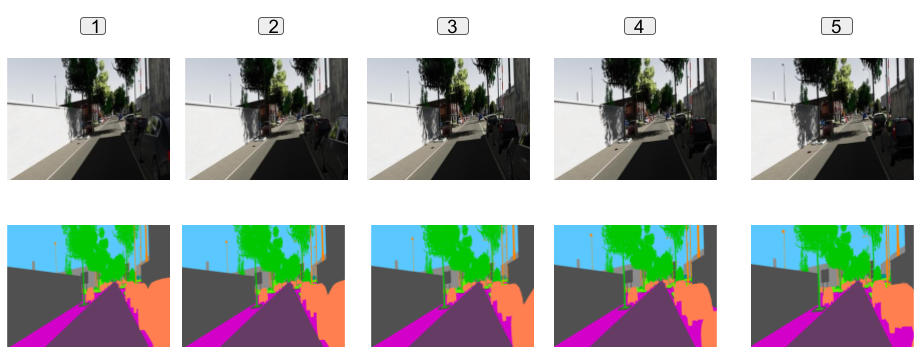
\includegraphics[width=14cm]{images/images_segm_vkitti.png}
		\caption{Sample of Virtual Kitti 2 dataset}
		\label{fig:sample_scannet_vkitti_2}
	\end{figure}

	\begin{figure}[h]
		\centering
		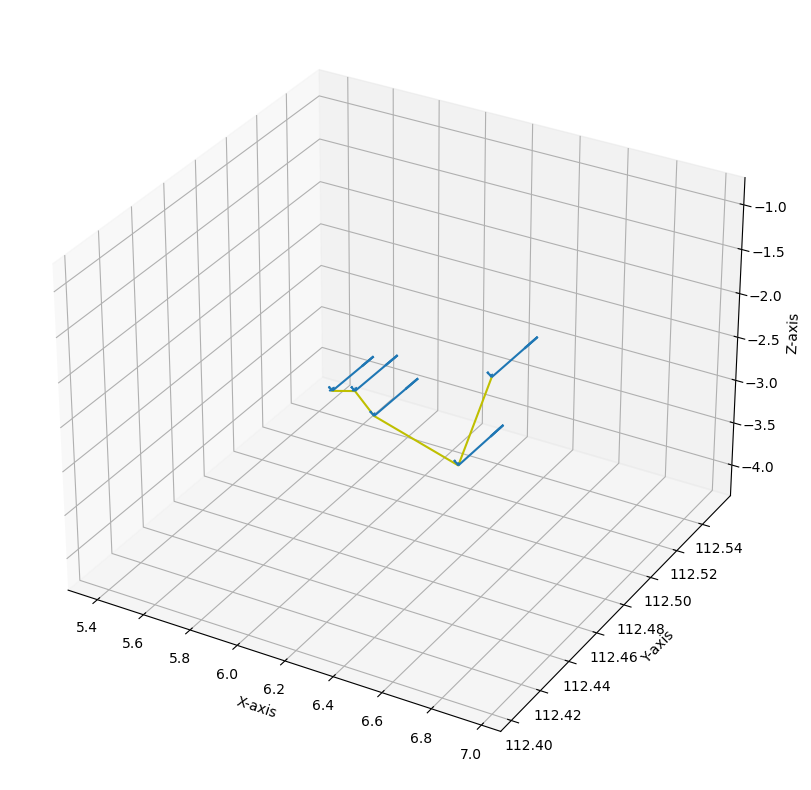
\includegraphics[width=14cm]{images/pose_viz_vkitti.png}
		\caption{Sample of Virtual Kitti 2 dataset}
		\label{fig:sample_pose_scannet_vkitti_2}
	\end{figure}
	
	\section{Data Collection and Preprocessing}
	
	The RGB-D scannet dataset can be downloaded from the python script sent to the user from the dataset development group, after submitting the agreement terms. The description and format of the dataset can be found at the github \ref{93_ScanNet}. Totally there are 1500 scans. Any specific scans, file types,  can be downloaded. There are multiple information regarding a scans in a file. These files are further processed to color, label, pose and depth data for each scans. More details is documented in the github \ref{94_ScanNet} repository. The raw rgb image is normalized before passing it into the model for quick convergence of learning. The input image is a 3 channel rgb data in .jpg format, the label is a single channel image in .png format with 40 classes in total, and pose data in text format. The pose data contains the rotation matrix and transnational vector in homogeneous matrix format. The vkitti dataset is also in the similar format. However, there are total of 15 classes in vkitti dataset. The raw rgb image, label and pose data is shown in the figure \ref{fig:scannet_vkitti}.

	\begin{figure}[h]
		\centering
		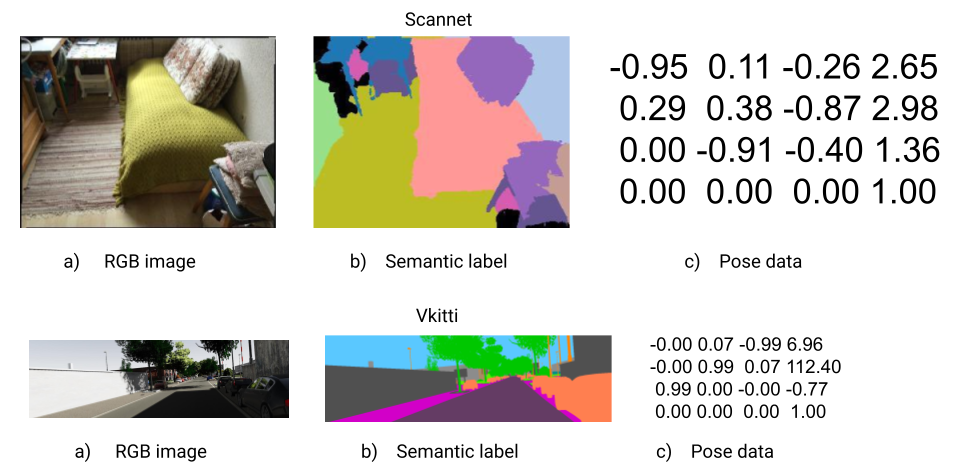
\includegraphics[width=14cm]{images/scannet_vkitti_data.png}
		\caption{RGB, Label and Pose dataset sample of scannet and vkitti data}
		\label{fig:scannet_vkitti}
	\end{figure}	
	
	
    \section{Experimental Design}
    
    The aim of the experiment is to incorporate temporal fusion in the latent space to understand the impact of past frames information fusion in the future frame segmentation prediction. The Unet model \ref{70_ronneberger2015u} perfectly suites to this experiment. Unet model consist of a encoder and a decoder network with latent space encoding in between. Three types of experiment were conducted with the unet model. In the first type plain vanilla unet model is taken in the second type of experiment unet model with gaussian process, third type is the unet model with Long Short Term Memory (LSTM). In the last two experiment the latent space encoding is subjected to temporal fusion by the gaussian process, and LSTM.   
    
    \subsection{U-Net Vanilla model}
    
    U-Net vanilla model is a simple semantic segmentation model, with encoder-decoder architecture. Encoder is a contracting path and decoder is a expanding path. The input image is fed into the encoder, made up of convolutional neural net. The architecture consist of two 3x3 2d convolutional layer followed by a rectified linear unit (ReLU) and batchnorm2d with 2d downsampling Maxpool layer. At every step of the convolutional block the number of out channels/ feature channel is doubled. Starting with 64 features in the first convolutional block output to 1024 feature at the downsampled fifth layer or the latent space encoding. The upsampling layer consist of a 2d convolution with halfed feature map at every step followed by concatenation of the corresponding feature map from the encoder path. The convolution2d consist of two 3x3 convolutions each followed by a ReLU function. At the final layer of the decoder, a 2d convolutional layer was introduced to map the previous convolutional block output to the predicted class labels. Totally there are 23 convolutional block in the entire network.    
	
	\begin{figure}[h]
		\centering
		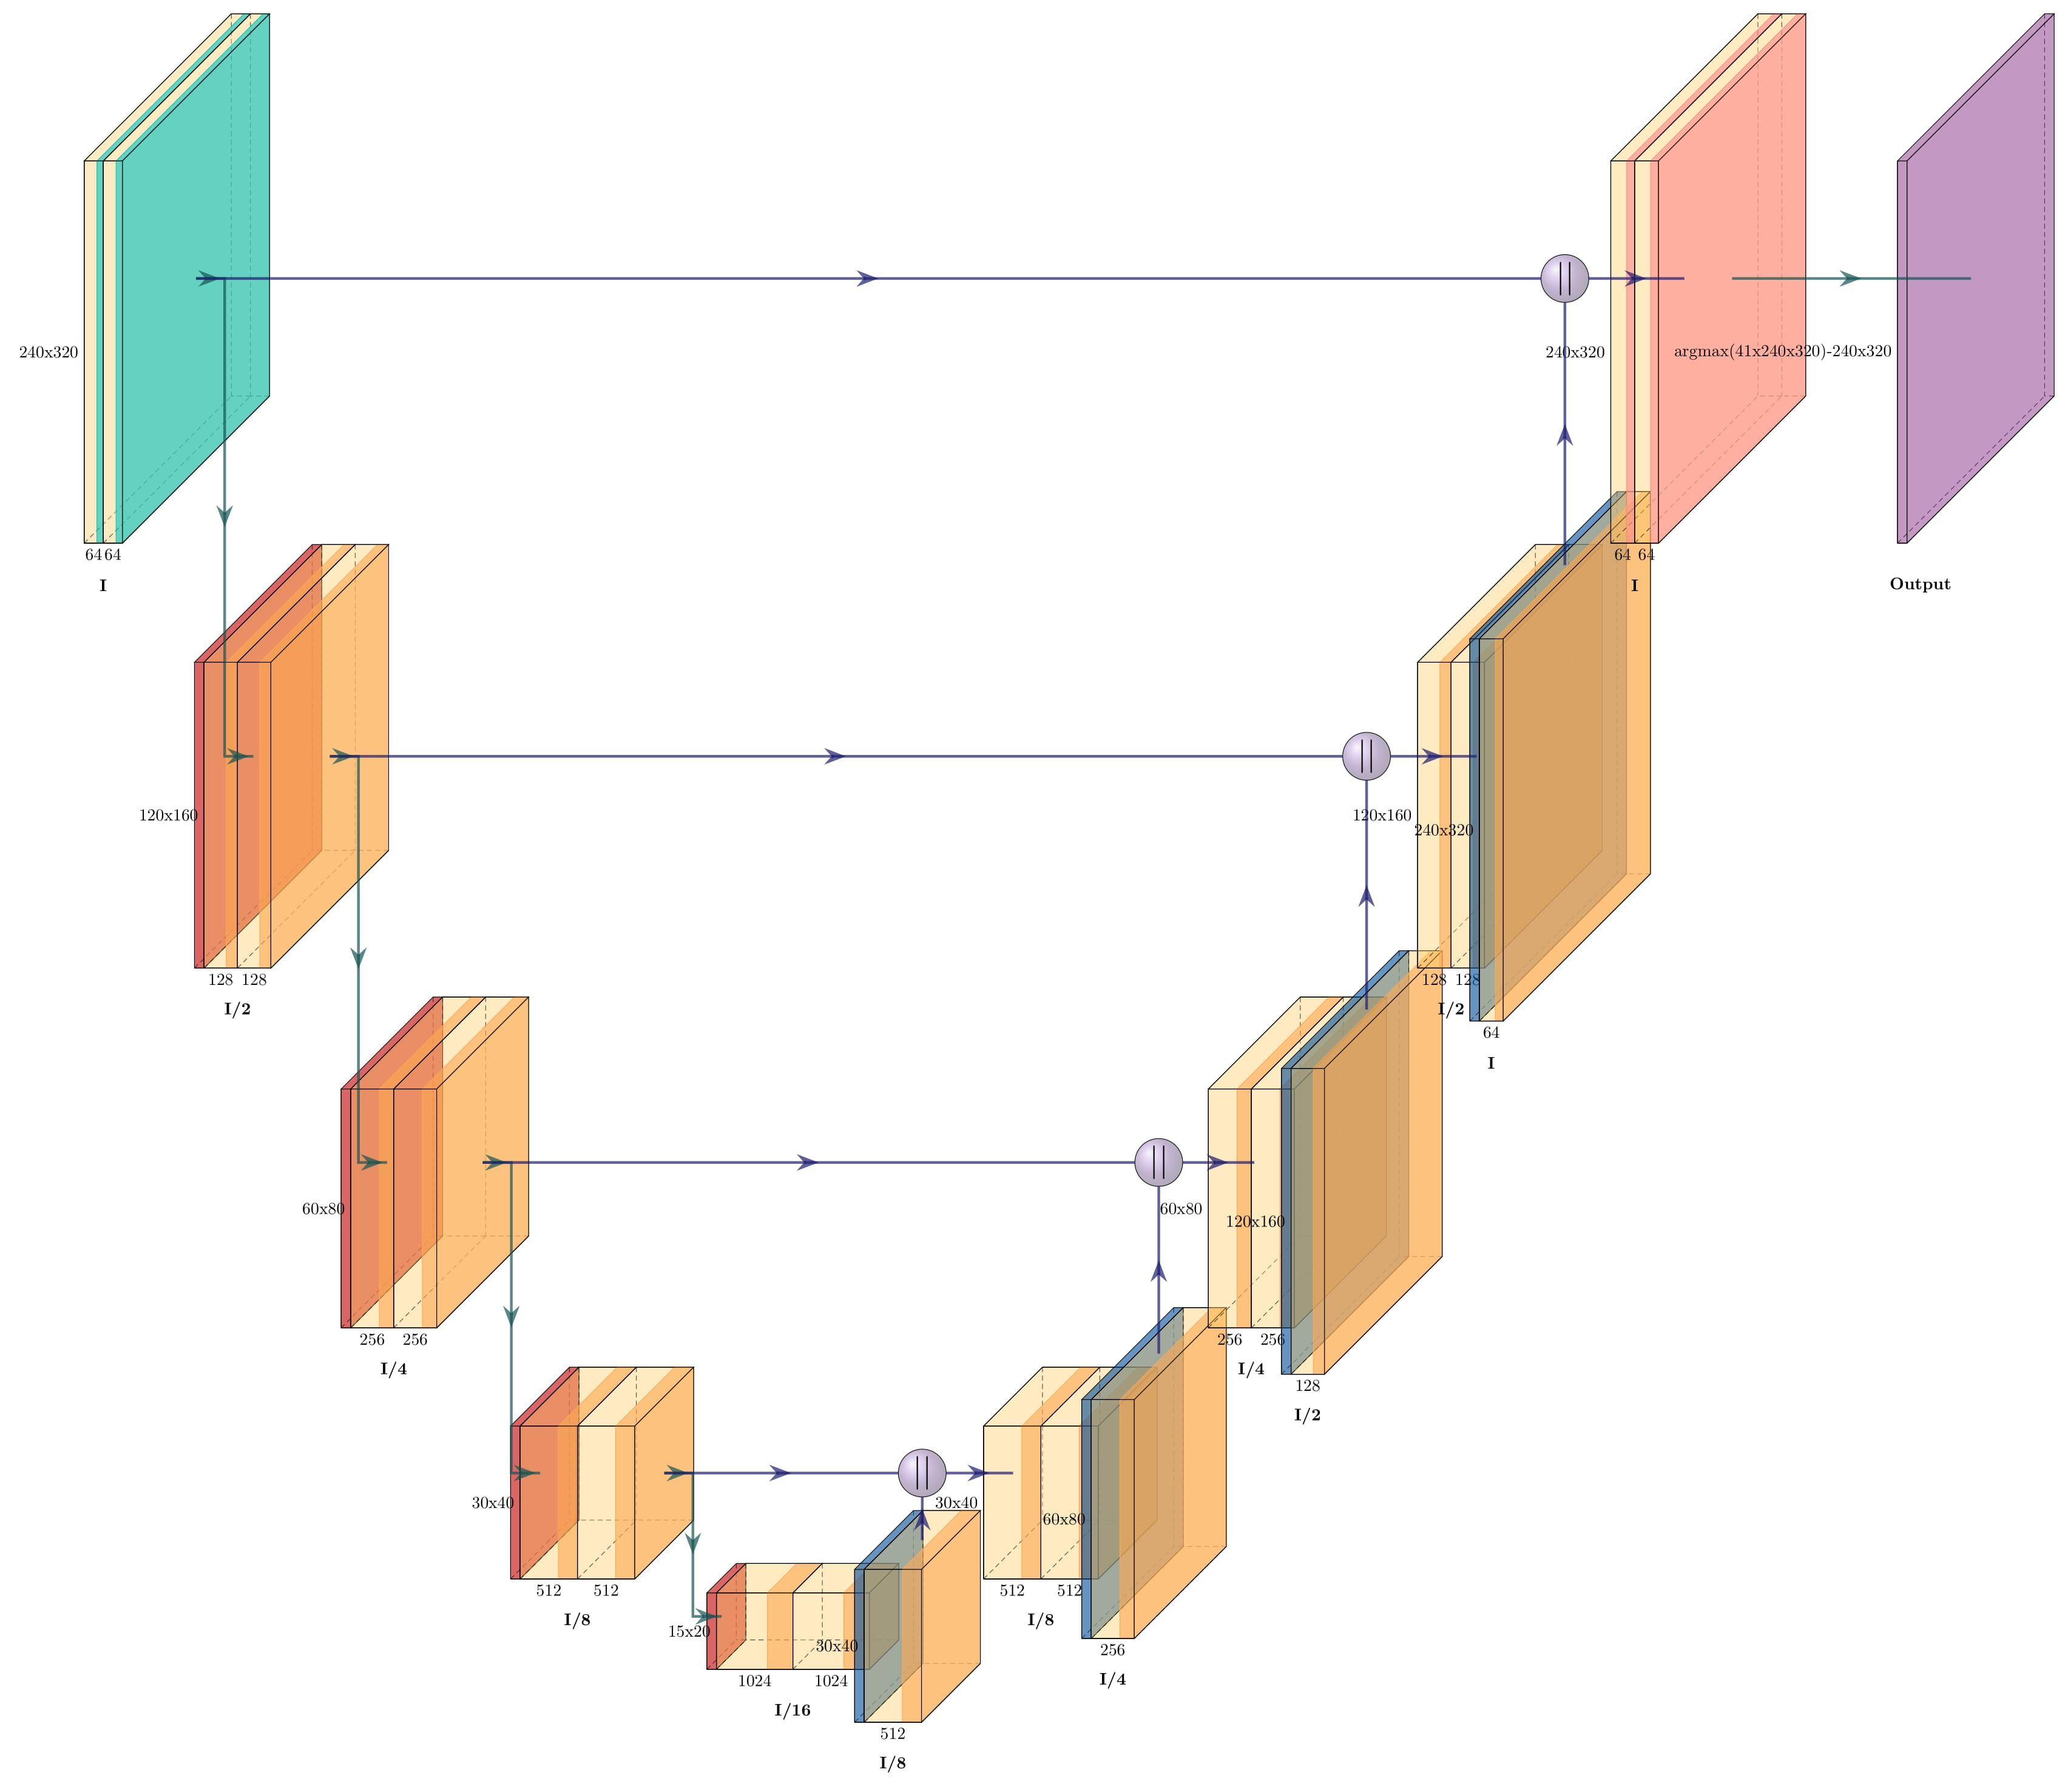
\includegraphics[width=14cm]{images/Unet.jpg}
		\caption{RGB, Label and Pose dataset sample of scannet and vkitti data}
		\label{fig:unet_model}
	\end{figure}
	
    \subsection{U-Net with Gaussian process}
    
    In the second type of experiment the latent space encoding of the U-Net model is taken and subjected to the gaussian process. The gaussian process make sure that the frames that are close to each other have similar latent space encodings. This is done by building the kernel of the gaussian process with distance matrix. A probabilistic prior on the latent space is defined that accounts for the prior knowledge that poses that are very close have similar latent space encoding than the poses that are very far from each other. This information is encoded in the covariance matrix. The distance measure between the camera poses is calculated with a metric to define the closeness. The distance between the camera poses is calculate with the help of work by Yuxin Hou et al \ref{52_hou2019multi} [02] and Mazzotti et al [97] \ref{95_mazzotti2016measure}. This measure the distance between the rigid body poses. The pose-distance measure between the two camera poses $P_i$ and $P_j$ is defined in equation \ref{eq:distance_matrix}. Where $t$ is the translation vector, $R$ is the rotational vector, $I$ is the identity matrix and $tr()$ is the trace of the matrix.  
    
    \begin{equation}
     D[P_i, P_j] = \sqrt{{||t_i - t_j||}^2 + \frac{2}{3} tr(I - R_i^TR_j)}
     \label{eq:distance_matrix}    
    \end{equation}
	
	The covariance function is defined from this distance matrix $D[P_i, P_j]$. The covariance function is chosen from the Matern class \ref{96_GPML}, \ref{97_williams2006gaussian} [97] [98] in equation \ref{eq:covariance_matrix}.  
	
	\begin{equation}
		k(P,P') = \gamma^2(1+\frac{\sqrt{3}D[P,P']}{l}exp(-\frac{\sqrt{3}D[P,P']}{l}))
		\label{eq:covariance_matrix}
	\end{equation}
	The hyperparameter $\gamma^2$ and $l$ define the magnitude and length-scale of the processes. Independent GP priors to all values in $Z_i$, and the output of the encoder is assumed to be the noise corrupted version of the expected latent space encodings. The GP regression model is defined from this initialization settings and defined in the equation \ref{eq:encode_output} \ref{eq:gp} [02]. The architecture of the unet model with gaussian process is depicted in the figure \ref{fig:unet_gp}.

	\begin{figure}[h]
		\centering
		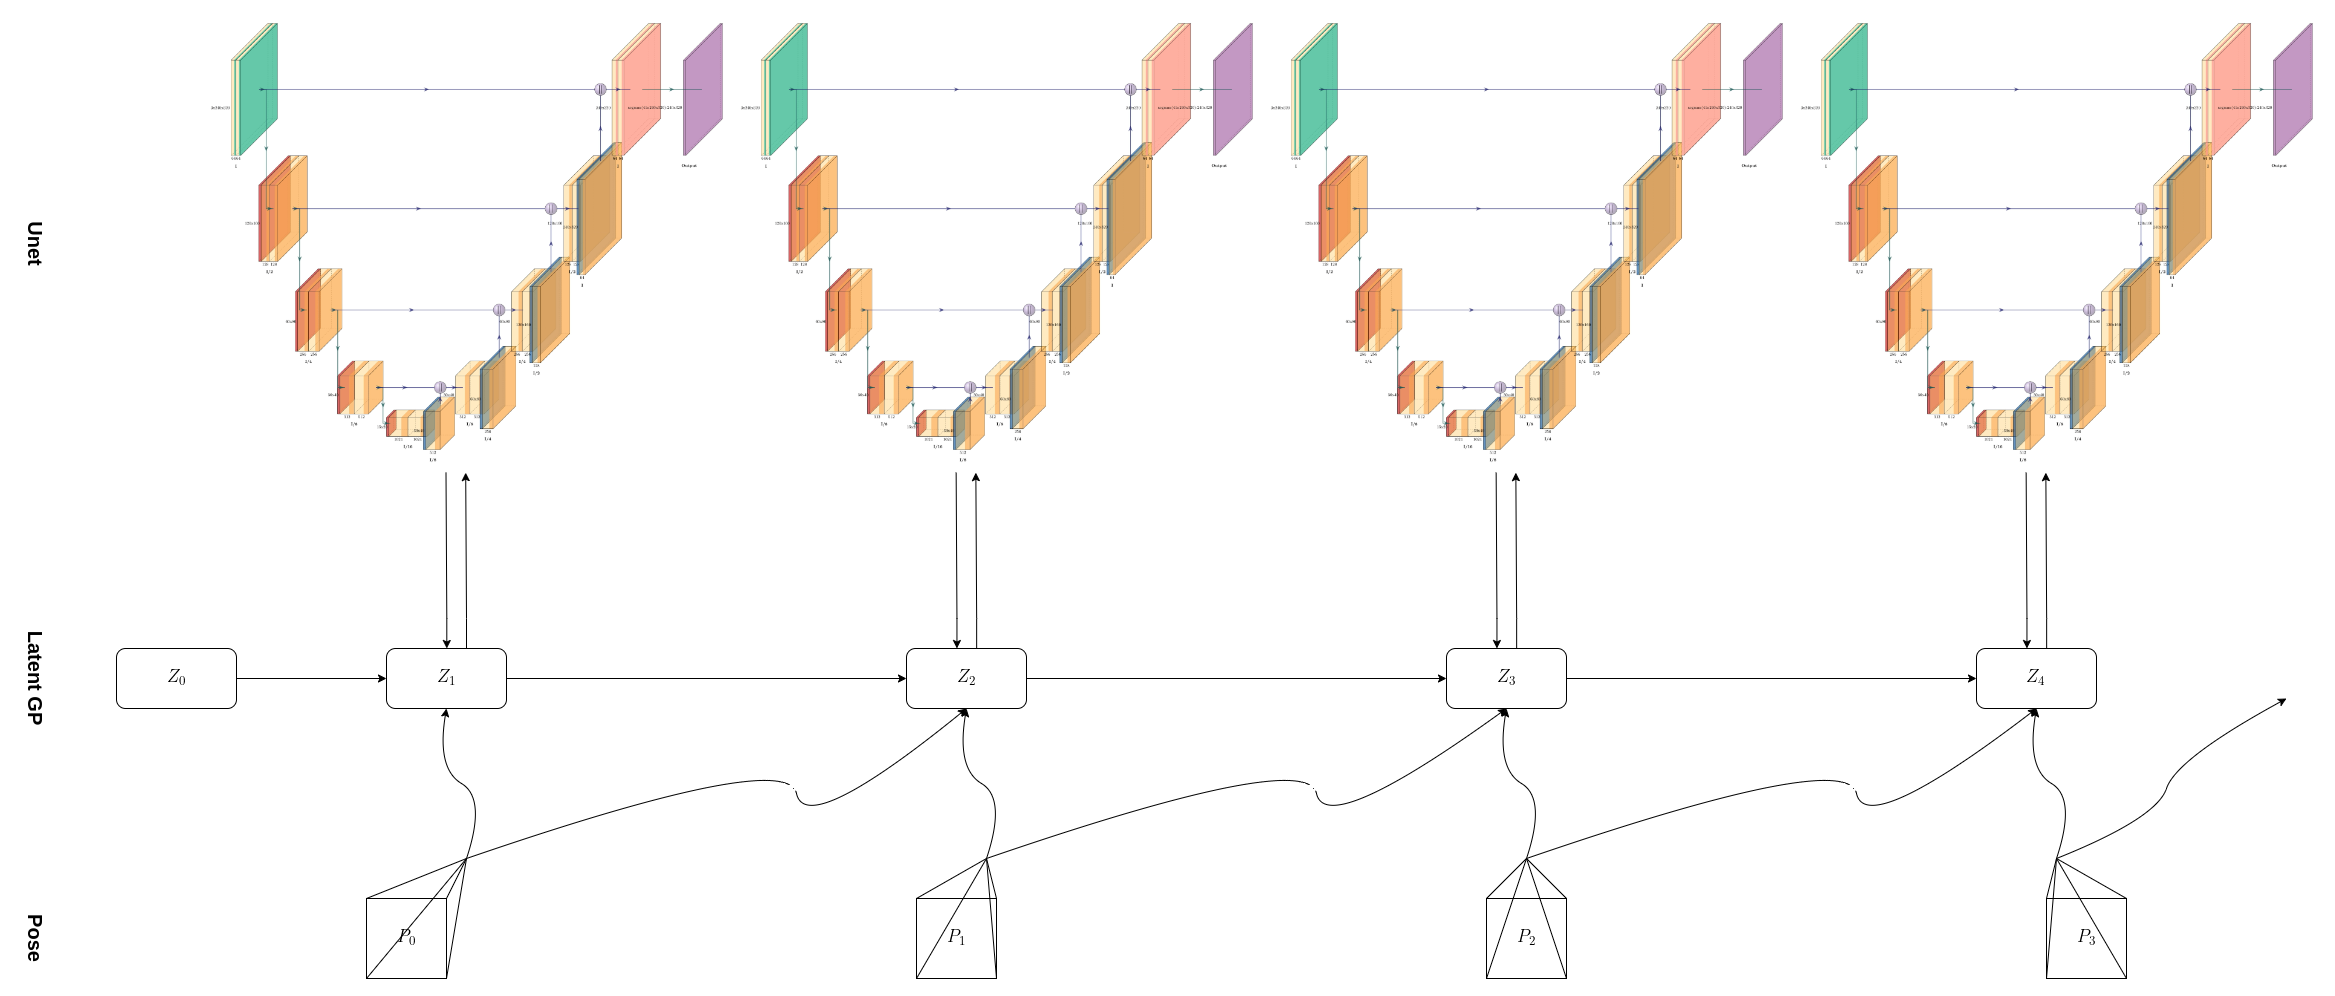
\includegraphics[width=14cm]{images/unet_gp.png}
		\caption{RGB, Label and Pose dataset sample of scannet and vkitti data}
		\label{fig:unet_gp}
	\end{figure}

	\begin{equation}
		z_j(t) \sim GP(0, k(P[t], P[t']))
		\label{eq:gp}
	\end{equation}
	
	\begin{equation}
		EncoderOutput = z_j(t_i)+ \epsilon_{j,i}, \epsilon_{j,i} \sim  N(0, \sigma^2)
		\label{eq:encode_output}
	\end{equation}
    
    
    \subsection{U-Net with Long Short Term Memory (LSTM)}
    
    In the third type of experiment, the U-Net model is subjected to the temporal fusion with the help of Long Short Term Memory (LSTM) by passing the latent space encoding onto the LSTM convolutional cell. The overlapping information in the consecutive frame data is passed onto the future frame prediction by incorporating the convolutional LSTM cell with the aim of improved performance and model the spatio temporal relations in comparison to the vanilla model. The partial scene geometry information from the previous frame is used in current step frame prediction. A hidden state propagation approach from LSTM method is used to pass the latent space information. The adaption of temporal fusion with LSTM is inspired from the work of Arda Düzçeker et al \ref{03_duzceker2021deepvideomvs}. The author introduced a convolutionalLSTM cell in the latent space to learn the shared information between the frames to predict the depth of objects present in a video sequence data. The convolutional LSTM cell is inspired from \ref{98_ConvLSTM}. The original LSTM version is explained in the article \ref{99_shi2015convolutional}. The hidden state $H$ and cell stae $C$ is initialized to a value. Let $X$ denotes the output of the bottleneck encoder network, then the logic to compute the hidden state and current state can be calculated as below (Courtesy of \ref{03_duzceker2021deepvideomvs})
    
    \begin{equation}
    	i_t = \sigma(w_{xi}*X_t+w_{hi}*H_{t-1})
    	\label{eq:it}
    \end{equation}
    \begin{equation}
		f_t = \sigma(w_{xf}*X_t+w_{hf}*H_{t-1})
		\label{eq:ft}
	\end{equation}    
    \begin{equation}
	 	o_t = \sigma(w_{xo}*X_t+w_{ho}*H_{t-1})
	 	\label{eq:ot}
 	\end{equation}   
    \begin{equation}
	    g_t = ELU(layernorm(w_{xg}*X_t+w_{hg}*H_{t-1}))
	    \label{eq:gt}
    \end{equation}
    \begin{equation}
	    C_t = layernorm(f_t \bigodot C_{t-1} +i_t \bigodot g_t)
	    \label{eq:Ct}
    \end{equation}
    \begin{equation}
	    H_t = o_t \bigodot ELU(C_t)
	    \label{eq:Ht}
    \end{equation}
    
    Where $*$ denotes the convolution, $\bigodot$ is the Hadamard product, $\sigma$ is the sigmoid activation function, $w$ are convolution filter weights. The pictorial representation of the same is presented in the Figure \ref{fig:unet_lstm}. Each frame of the sequence video is passed onto the bottleneck U-net model in order and prediction is made for individual frames. The output from the encoder network is passed through LSTM cell. The output from first LSTM cell act as the input to the next LSTM cell computation, thereby it carries the learned information forward from one frame computation to the next frame computation.   
    
	\begin{figure}
		\centering
		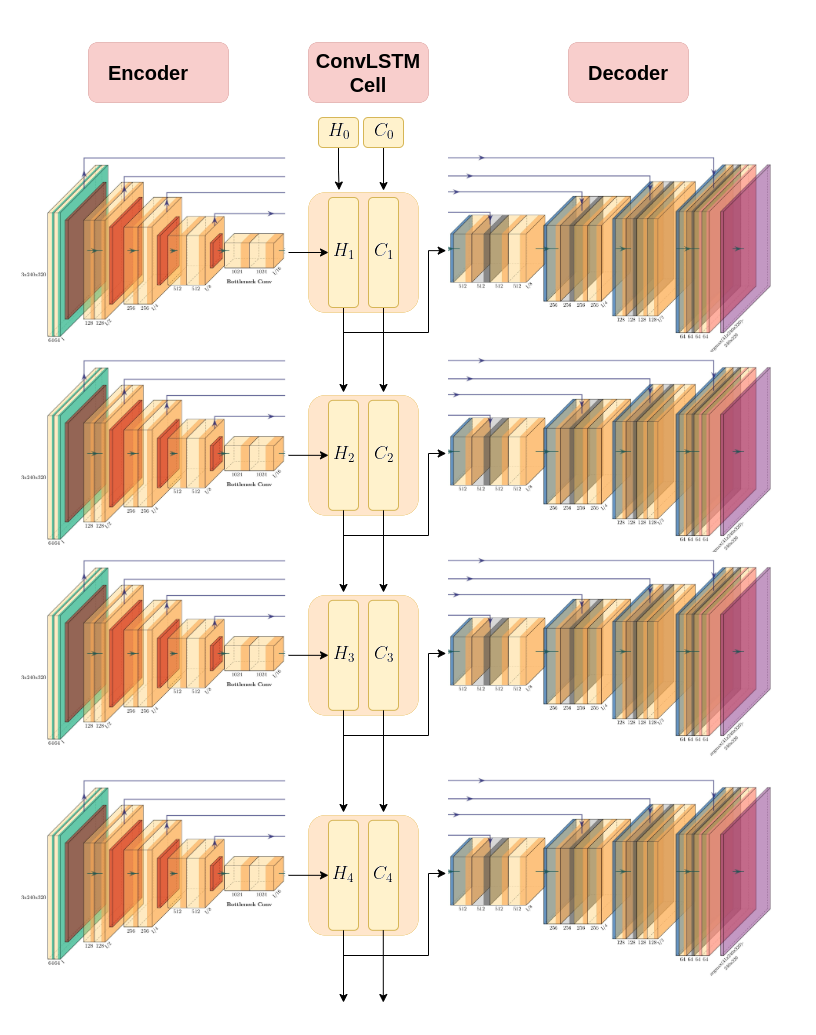
\includegraphics[width=14cm]{images/unet_lstm.png}
		\caption{Unet with ConvLSTM cell}
		\label{fig:unet_lstm}
	\end{figure}     
        
    \section{Training and Evaluation Pipeline}
    
    Datasets are splitted into training and evaluation set. During the training phase the image, label and pose paths are added into a list in order and then passed onto the dataloader. The image data is read and normalized.  Experiment is conducted with different number of classes by merging the classes. This is done in labels  processing stage. A model is initialized with different parameter settings. The processed image, label and pose data is passed onto the initialized model. A loss criteria is defined to compute the losses. Loss is computed from the ground truth value and the model prediction. Back propagation from the loss is calculated followed by the optimization step. In the final stage the loss and model is saved. The dataloader loads data in batches. The process is repeated until all the data in the dataloader iterate through entire data once. The entire process is repeated for different number of epochs. Model performance is monitored during each run of the epoch and stopped once the loss reaches a small values and model fits to the training data. 
    
    During the evaluation process the evaluation dataset path is stored in the list. The individual list contains Image, Label and Pose path information. Since the dataset is a continuous sequence data, the path of the data stored in the list are in order. In most of the cases there is a overlapping information between the consecutive frames. In the evaluation dataset are passed onto the dataloader. Images are normalized from this dataloader and labels are processed as per the requirement set by the experiments. Pose information is in text format. The text data is read and passed to a list and returned by the dataloader. The trained model is loaded and the processed data from the dataloader is passed onto the model. The predicted output from the model is evaluated against the evaluation metric and the results are saved.      
    
    
   	\begin{figure}
    	\centering
    	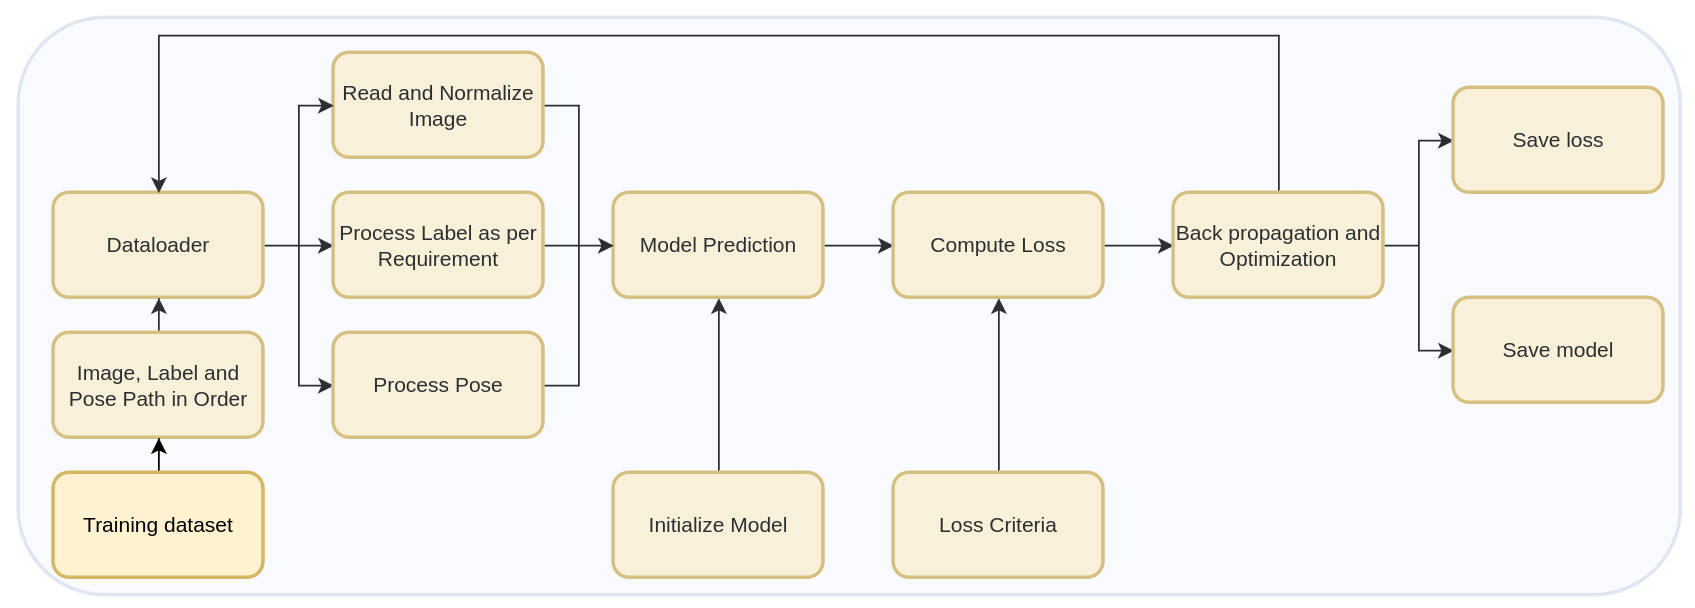
\includegraphics[width=14cm]{images/training.png}
    	\caption{Training pipeline}
    	\label{fig:unet_training}
    \end{figure}

	\begin{figure}
		\centering
		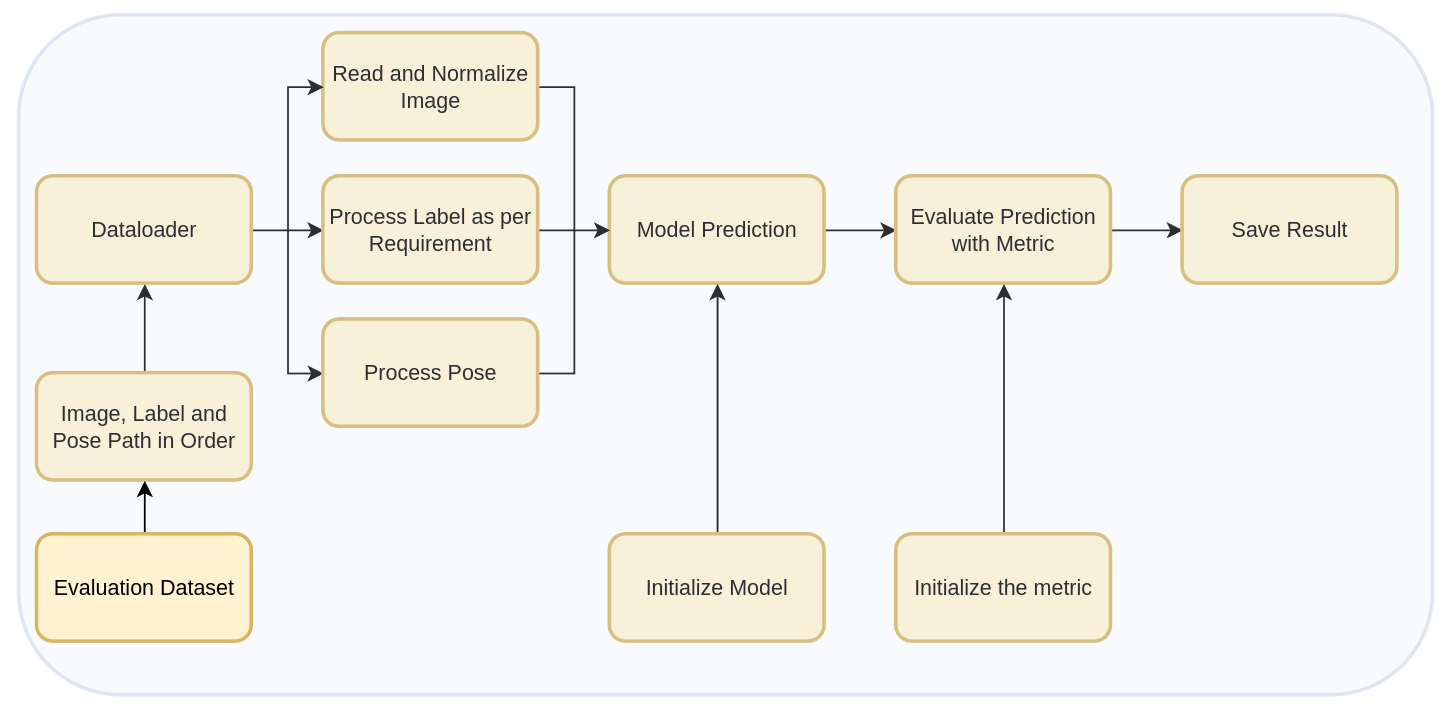
\includegraphics[width=14cm]{images/evaluation.png}
		\caption{Evaluation pipeline}
		\label{fig:unet_evaluation}
	\end{figure}
    
    \section{Hardware Configuration}
    
    NVIDIA GeForce RTX 3070 Laptop GPU, 8192 MB
    Tesla T4, 12680 MB, Google Colab
    Nvidia Tesla V100 PCIe GPU with 5120 Cuda cores and 640 Tensor cores, 16 GB HBM2 memory University cluster
    
\end{document}
